% !TEX root = index.tex

\section{Geometric Meaning of Curvature}

\subsection{Mean Curvature}
  The Mean Curvature shows up in physics while studying soap films. At a point on a soap film the difference between the pressure on two sides is proportional to the mean curvature of the surface at that point. This is called the \textbf{Young-Laplace equation}.
  \begin{align*}
    \Delta (\mbox{pressure}) \propto H
  \end{align*}
  If the soap film does not bound a volume, for example, if it is bounded by a curve then the pressure on both the sides is the same and hence the mean curvature at every point must be 0. Such surfaces are called \textbf{minimal surfaces}, minimal because these surfaces also have the minimal surface area of all the surfaces bounding the curve. The study of minimal surfaces is a very active area of research in geometry.
  \begin{figure}[H]
    \centering
    \begin{subfigure}[t]{0.495\textwidth}
      \centering
      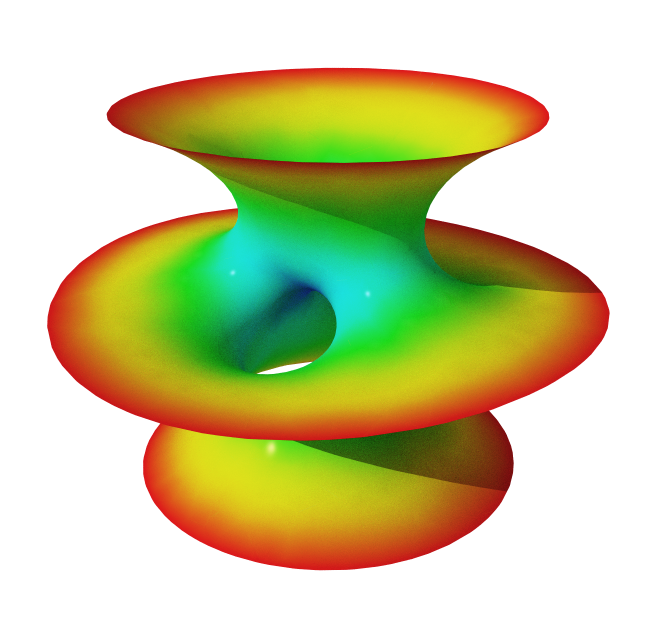
\includegraphics[width=6cm]{Minimal_Surface_1}
    \end{subfigure}
    \begin{subfigure}[t]{0.495\textwidth}
      \centering
      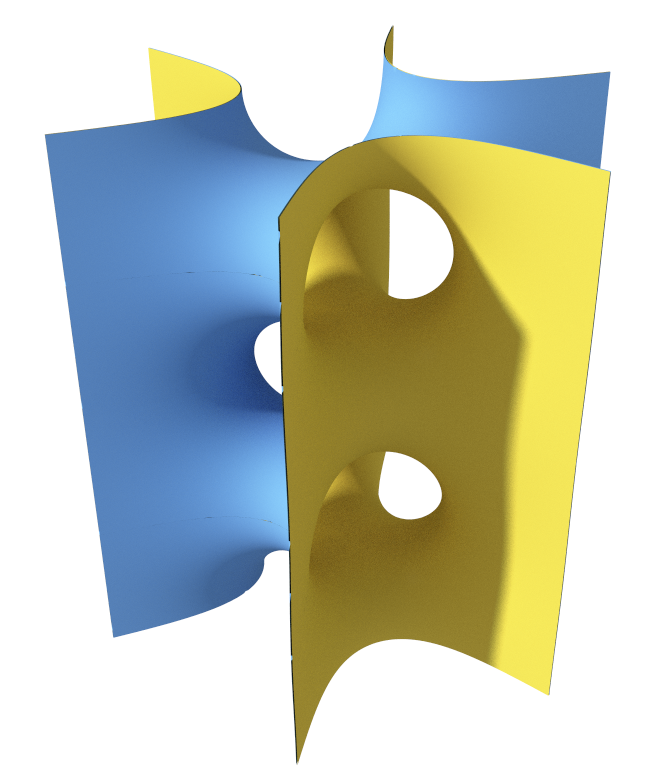
\includegraphics[width=6cm]{Minimal_Surface_2}
    \end{subfigure}
    \caption{Examples of minimal surfaces. The Mean Curvature at \emph{every} non-boundary point is 0 and hence at every point the surface looks like the perfect potato chip. Images from \href{https://en.wikipedia.org/wiki/Minimal_surface}{Wikipedia}.}
  \end{figure}

\subsection{Gaussian Curvature}
  The Gaussian Curvature is much more subtle and has several interpretations.

  \begin{definition}
    For a surface $S$ the \textbf{geodesic distance} $d_S(p,q)$ between two points $p,q \in S$ is defined to be the shortest length of the curve on the surface $S$ that connects $p$ to $q$.
  \end{definition} For example, on a plane the geodesic distance is simply the Euclidean distance. On a sphere, the geodesic distance between two points is the length of the arc of the great circle connecting them.
  \begin{figure}[H]
    \centering
      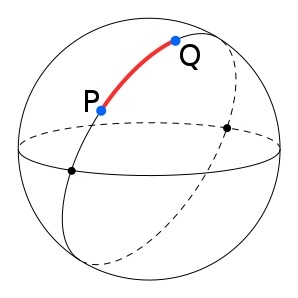
\includegraphics[width=3cm]{great_circle}
    \caption{The geodesic distance between two points on a sphere is the length of the arc of the great circle connecting them. Image from \href{https://en.wikipedia.org/wiki/Great-circle_distance}{Wikipedia}.}
  \end{figure}

  \begin{definition}
    The \textbf{geodesic ball} of radius $r$ centered at a point $p \in S$ is the set of points which are at a geodesic distance of at the most $r$ from $p$
    \begin{align*}
      B_r(p) := \{ x \in S : d_S(x,p) \le r\}
    \end{align*}
  \end{definition}
We'll assume the following theorem without proof.
  \begin{thm}
    The Gaussian curvature of $S$ at $p$ equals
    \begin{align*}
      K &= 3 \lim \limits_{r \rightarrow 0} \dfrac{2 \pi r - \mbox{length of } \partial B_S(p,r) }{\pi r^3}
    \end{align*}
  \end{thm}
\begin{cor}
  \label{thm:geodesics}
  The Gaussian curvature can be computed by measuring distances on the surface (without knowing anything about the ambient space).
\end{cor}
This leads directly to the next theorem.

  \subsubsection{Theorema Egregium}
  We can take a sheet of paper and roll into a cylinder without stretching or compressing the sheet.\footnote{Neglect the \emph{thickness} of the paper.} Such a map is called an \textbf{isometry}.



  \begin{definition}
    A smooth map $\phi: S \rightarrow S'$ is called an \textbf{isometry} if
    \begin{align*}
      d_S(p,q) = d_{S'}(\phi(p),\phi(q))
    \end{align*}for any two points $p,q \in S$.
  \end{definition}
  \noindent The map that sends a plane to a cylinder is an example of such an isometry.
  \begin{thm}[Theorema Egregium]
    \label{thm:theorema}
    If there exists an isometry $\phi: S \rightarrow S'$ between two surfaces then the Gaussian curvature of $S$ at $p \in S$ equals the Gaussian curvature of $S'$ at $\phi(p)$.
  \end{thm}
  \begin{proof}
    This is a direct consequence of Corollary \ref{thm:geodesics}. It is possible to measure the Gaussian curvature using only the geodesic distances and geodesic distances are preserved under isometry.
  \end{proof}
  This theorem is interpreted as saying that the Gaussian curvature is \emph{intrinsic} to a surface.


\subsubsection{Gauss Map}
\begin{figure}[H]
  \centering
    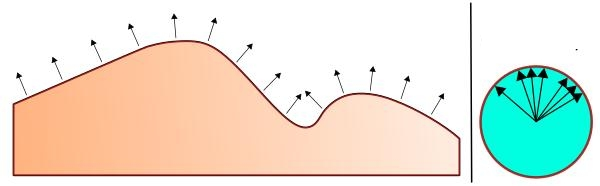
\includegraphics[width=8cm]{Gauss_map}
  \caption{The unit normal vector $\vec n$ defines a map from the surface to the unit sphere $\vec n : S \rightarrow S^2$. Image from \href{https://en.wikipedia.org/wiki/Gauss_map}{Wikipedia}.}
\end{figure}
Let $\vec n$ denote a continuously varying unit normal vector field on the surface $S$. There are two possibly choices for $\vec n$, we just pick one. We can think of $\vec n$ as a map, called the \textbf{Gauss map} from $S$ to the unit sphere $S^2$. Then,
\begin{align*}
  K &= \lim \limits_{r \rightarrow 0} \dfrac{\mbox{area of } \vec n (B_r(p)) }{\mbox{area of } B_r(p) }
\end{align*}

\subsubsection{Gauss-Bonnet theorem}
Gaussian curvature has a topological significance as well. If $S$ is a closed surface then
\begin{thm}
  The total Gaussian Curvature
  \begin{align*}
    \int \limits_S K \: dA = 2 \pi \chi(S)
  \end{align*}
  where $\chi(S)$ denotes the Euler characteristic of the surface.
\end{thm}

\subsection{Final Remarks}
The methods that we've described only define the various curvatures for \emph{embedded} surfaces. In general, because the Gaussian curvature can be computed by measuring Geodesic distances it is possible to define the Gaussian curvature (but not the principal and mean curvatures) for manifolds with a metric (also called Riemannian manifold).
